\chapter{Overleaf \\
\small{\textit{-- Spurthi Setty}}
\index{bugzilla} 
\index{Chapter!Overleaf}
\label{Chapter::Overleaf}}

\section{How to compile this chapter}
Add to your preamble and compile with shell-escape to enable \texttt{minted}:
\begin{minted}[fontsize=\small]{latex}
\usepackage{xcolor}
\usepackage{minted}
\setminted{fontsize=\small,breaklines=true}
% Compile with:  latexmk -pdf -shell-escape main.tex
\end{minted}

\section{Context}
We deployed \textbf{Overleaf Community Edition} on an existing DigitalOcean droplet that already served another site on \url{http://167.99.54.162:8080}. To avoid port conflicts, Overleaf was mapped to port \texttt{8090}.

\section{Prerequisites (Ubuntu 22.04/24.04)}
\begin{minted}[fontsize=\small]{bash}
# optional: install Docker Engine + compose plugin (if not present)
apt-get update -y
apt-get install -y ca-certificates curl gnupg lsb-release
install -m 0755 -d /etc/apt/keyrings
curl -fsSL https://download.docker.com/linux/ubuntu/gpg | gpg --dearmor -o /etc/apt/keyrings/docker.gpg
chmod a+r /etc/apt/keyrings/docker.gpg
echo "deb [arch=$(dpkg --print-architecture) signed-by=/etc/apt/keyrings/docker.gpg] \
https://download.docker.com/linux/ubuntu $(lsb_release -cs) stable" \
| tee /etc/apt/sources.list.d/docker.list > /dev/null
apt-get update -y
apt-get install -y docker-ce docker-ce-cli containerd.io docker-buildx-plugin docker-compose-plugin
systemctl enable --now docker

# sanity
docker --version
docker compose version
\end{minted}

\section{Baseline deployment}
\subsection{Create working directory}
\begin{minted}{bash}
mkdir -p /opt/overleaf
cd /opt/overleaf
\end{minted}

\subsection{Open firewall}
\begin{minted}{bash}
ufw allow OpenSSH
ufw allow 8090/tcp
ufw --force enable
ufw status
\end{minted}

\subsection{Initial \texttt{docker-compose.yml}}
We used \texttt{sharelatex/sharelatex} (the Overleaf CE image) with MongoDB and Redis. Note the \textbf{Overleaf-branded} env vars and the \textbf{new data path} \texttt{/var/lib/overleaf}.
\begin{minted}[fontsize=\small]{yaml}
services:
  mongo:
    image: mongo:6.0
    restart: unless-stopped
    volumes:
      - overleaf_mongo_data:/data/db

  redis:
    image: redis:7
    restart: unless-stopped
    command: ["redis-server","--appendonly","yes"]
    volumes:
      - overleaf_redis_data:/data

  sharelatex:
    image: sharelatex/sharelatex:latest
    container_name: sharelatex
    restart: unless-stopped
    depends_on:
      - mongo
      - redis
    environment:
      OVERLEAF_SITE_URL: "http://167.99.54.162:8090"
      OVERLEAF_MONGO_URL: "mongodb://mongo:27017/sharelatex"
      OVERLEAF_REDIS_HOST: "redis"
    ports:
      - "8090:80"
    volumes:
      - overleaf_app_data:/var/lib/overleaf

volumes:
  overleaf_mongo_data:
  overleaf_redis_data:
  overleaf_app_data:
\end{minted}

\subsection{Start the stack}
\begin{minted}{bash}
cd /opt/overleaf
docker compose pull
docker compose up -d
docker compose ps
\end{minted}

\section{Issues encountered and exact fixes}
Below are the exact errors we hit and the precise commands that resolved them on this host.

\subsection{(A) Wrong image / registry hiccup}
\textit{Symptom:} Pull errors for \texttt{ghcr.io/overleaf/overleaf} (access denied/registry auth).\\
\textit{Fix:} Switch to Docker Hub image \texttt{sharelatex/sharelatex}.
\begin{minted}{bash}
# if your compose ever referenced ghcr, replace it with Docker Hub image
sed -i 's#ghcr.io/overleaf/overleaf:latest#sharelatex/sharelatex:latest#' docker-compose.yml
\end{minted}

\subsection{(B) Legacy bind mount path: \texttt{/var/lib/sharelatex}}
\textit{Symptom:} Container logs show rebranding guard refusing to start due to old path.\\
\textit{Fix:} Use the new path \texttt{/var/lib/overleaf} in the bind mount.
\begin{minted}{bash}
sed -i 's#/var/lib/sharelatex#/var/lib/overleaf#g' docker-compose.yml
\end{minted}

\subsection{(C) Legacy env var names: \texttt{SHARELATEX\_*}}
\textit{Symptom:} \texttt{000\_check\_for\_old\_env\_vars\_5.sh} refuses startup, listing \texttt{SHARELATEX\_MONGO\_URL}, \texttt{SHARELATEX\_REDIS\_HOST}, \texttt{SHARELATEX\_SITE\_URL}.\\
\textit{Fix:} Rename to the Overleaf-branded variants.
\begin{minted}{bash}
sed -i -E 's/SHARELATEX_MONGO_URL/OVERLEAF_MONGO_URL/g; \
s/SHARELATEX_REDIS_HOST/OVERLEAF_REDIS_HOST/g; \
s/SHARELATEX_SITE_URL/OVERLEAF_SITE_URL/g' docker-compose.yml

# if you had a .env with legacy keys, update it too
sed -i 's/SHARELATEX_SITE_URL/OVERLEAF_SITE_URL/' .env 2>/dev/null || true
\end{minted}

\subsection{(D) Connection reset / app crash loop due to Mongo transactions}
\textit{Symptom:} Logs show: \texttt{Transaction numbers are only allowed on a replica set member or mongos}.\\
\textit{Cause:} Overleaf 5+ expects MongoDB with transactions support (i.e., a replica set), even for a single node.\\
\textit{Fix:} Run Mongo as a single-node replica set and update the connection string.

\paragraph{Step D1: Add override to enable replica set and connection string}
\begin{minted}{bash}
cat > docker-compose.override.yml <<'YML'
services:
  mongo:
    command: ["mongod","--replSet","rs0","--bind_ip_all"]
  sharelatex:
    environment:
      OVERLEAF_MONGO_URL: "mongodb://mongo:27017/sharelatex?replicaSet=rs0"
YML
\end{minted}

\paragraph{Step D2: Recreate the stack}
\begin{minted}{bash}
docker compose down
docker compose up -d
\end{minted}

\paragraph{Step D3: Initialize the replica set (one-time)}
\begin{minted}{bash}
# try mongosh (6.x); fallback to legacy mongo shell if needed
docker exec overleaf-mongo-1 bash -lc \
  'mongosh --quiet --eval "rs.initiate({_id:\"rs0\", members:[{_id:0, host:\"mongo:27017\"}]})"' \
  || docker exec overleaf-mongo-1 bash -lc \
  'mongo --quiet --eval "rs.initiate({_id:\"rs0\", members:[{_id:0, host:\"mongo:27017\"}]})"'
\end{minted}

\paragraph{Step D4: Verify replica set is healthy}
\begin{minted}{bash}
docker exec overleaf-mongo-1 bash -lc 'mongosh --quiet --eval "rs.status().ok"' \
  || docker exec overleaf-mongo-1 bash -lc 'mongo --quiet --eval "rs.status().ok"'
# expect: 1
\end{minted}

\subsection{(E) Optional: tune kernel warning from Redis}
\begin{minted}{bash}
# not required for functionality, but silences Redis warning
sysctl -w vm.overcommit_memory=1
echo 'vm.overcommit_memory=1' >> /etc/sysctl.conf
\end{minted}

\section{Verification commands we used}
\begin{minted}{bash}
# container status
cd /opt/overleaf
docker compose ps

# app health (host)
curl -I http://localhost:8090
curl -sS http://localhost:8090/health_check || true

# service status inside the container (runit + port 80)
docker exec -it sharelatex bash -lc 'sv status nginx; sv status sharelatex; ss -tlnp | grep :80 || true'

# logs (when diagnosing)
docker compose logs --tail=200 sharelatex
\end{minted}

\section{Accessing the site}
First-time admin setup (\textit{Launchpad}):
\url{http://167.99.54.162:8090/launchpad}
After creating the admin, use the main URL:
\url{http://167.99.54.162:8090}

\section{Maintenance cheatsheet}
\begin{minted}{bash}
# restart
cd /opt/overleaf
docker compose down
docker compose up -d

# upgrade images (occasional)
docker compose pull && docker compose up -d

# view logs
docker compose logs -f sharelatex

# backups of volumes (quick tar via busybox)
mkdir -p /opt/overleaf/backups
cd /opt/overleaf
for v in overleaf_app_data overleaf_mongo_data overleaf_redis_data; do
  docker run --rm -v ${v}:/data -v $(pwd)/backups:/backup busybox \
    tar czf /backup/${v}_$(date +%F).tar.gz /data
done
\end{minted}

\section{Final status}
After applying fixes (B) path update, (C) env var rename to \texttt{OVERLEAF\_*}, and (D) enabling a single-node Mongo replica set, Overleaf CE started cleanly and became reachable at \url{http://167.99.54.162:8090}. The \texttt{/launchpad} route was used to create the initial admin account.

\begin{figure}
    \centering
    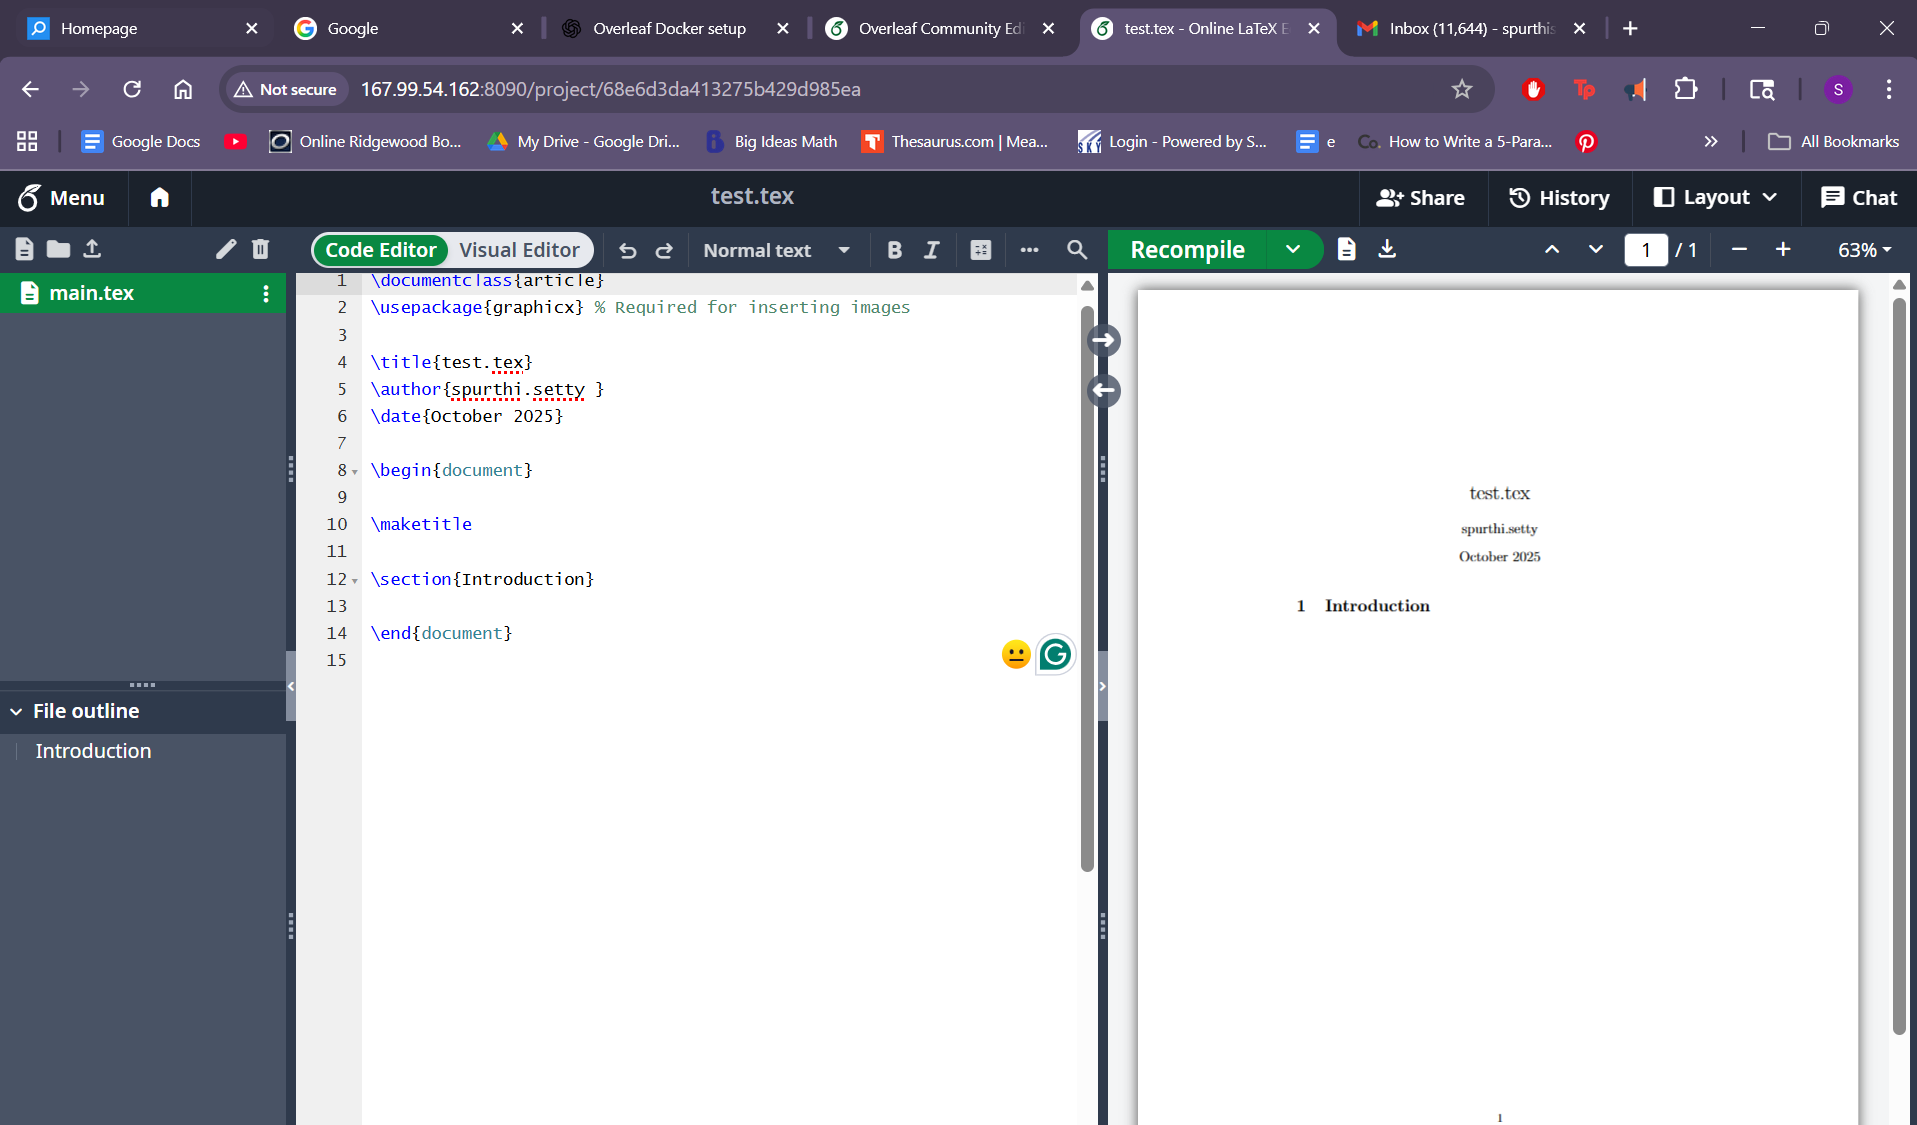
\includegraphics[width=0.9\linewidth]{png/overleaf.png}
    \caption{Screenshot of Compiled File at \url{http://167.99.54.162:8090}}
    \label{fig:placeholder}
\end{figure}


\section{Creating a New User Account}

To create a new account manually from the administrator dashboard, follow these steps:

\begin{enumerate}
  \item \textbf{Login as an administrator.}
        Open your Overleaf instance and sign in with your admin credentials.
  \item \textbf{Open the Manage Users panel.}
        Click on your profile icon at the top right corner and select \texttt{Manage Users}.
  \item \textbf{Register the new user.}
        In the user management form, enter the email address of the new user and click \texttt{Register}.
  \item \textbf{Access the Set Password page.}
        Copy the \texttt{Set Password} URL generated for that user and paste it into your browser.
  \item \textbf{Set a new password.}
        The page will prompt you to create a new password for the account. Enter the desired password and confirm it.
  \item \textbf{Activate and log in.}
        After setting the password, click \texttt{Activate}. The user can now log in using the new credentials.
\end{enumerate}
